\newcommand{\bmweb}{\psi}
\newcommand{\toinP}{\overset{\P}\to}
\newcommand{\statementoflemresampledetosampled}{$\resamplede \toinP \sampled$ as $\epsilon \to 0$}
{
\section{Recovering the Brownian web from its horizontal half-planes}

\label{recovering-from-half-planes}\TODO{}{improper labeling convention - put sec:}

\TODO{}{Should we move the definitions to an earlier section?}

\newcommand{\restrictupper}{\mathcal{R}_{+}}

  For any path $f$ we write $\restrictupper(f)$ for $f$ stopped at the
  first time it is outside the upper half-plane.
  $\restrictupper(t \mapsto \web{s}{t}{x})$ is therefore the trajectory of the
  web $\webnoargs$ started at the point $(s,x)$ and stopped at the first
  time it is outside the upper half-plane.

  Write $\wholefield$ for the $\sigma$-field generated by the
  whole web, i.e.\ by all its trajectories $t \mapsto \web{s}{t}{x}$.
  We define $\upperhp$ to be the $\sigma$-field generated by the
  collection of paths $\{\restrictupper(t \mapsto \web{s}{t}{x} : s,x
  \in \R \}$, and define $\lowerhp$ analogously.
  Note that $\upperhp$ and $\lowerhp$ are independent by the definition of
  a system of $n$-coalescing Brownian motions.

  We are now ready to state a formal version of Theorem
  \ref{thm:informal-recovering-from-half-planes}.

\begin{theorem}\label{thm:recoveringfromhalfplanes}
  $\wholefield = \twostrips$
\end{theorem}

The only difficulty is to show that $\wholefield \subseteq \twostrips$,
because the reverse inclusion follows directly from the definitions.
Fix a starting point $(s,x)$ and write $\sampled$ for the random
process $t \mapsto \web{s}{t}{x}$ (which is a Brownian motion).  Now
$\wholefield$ is generated by processes of the form $\sampled$, so
our theorem reduces to the following lemma.

\begin{lemma}
  \label{lem:sampled-twostrip-meas}
  $\sampled$ is $\twostrips$-measurable.
\end{lemma}

Equivalently, by using trajectories starting on the upper half-plane
which ``die out'' when they hit $0$ and trajectories starting on
the lower half-plane which ``die out'' when they hit $0$ as well we
can recover all of the web's trajectories.
To see that Lemma \ref{lem:sampled-twostrip-meas} is non-trivial,
observe that the following does not work. We cannot recover a web's
trajectory by following it on, say, the upper half-plane until it
hits 0, then following a trajectory starting from that point on the
lower half-plane. The reason for this is that trajectories starting at
0 ``die out'' immediately. Observe that this problem does not arise when
trying to use information about two overlapping half-planes, so it is
not difficult to recover the web from such.
\TODO{}{Check grammar}

To overcome this problem, for every starting point, say in the upper
half-plane, we define the following process. While the process is in
the upper half-plane, it follows the upper half-plane web until it hits
$0$, at which point it starts to follow a Brownian motion entirely
independent of the web. It follows this Brownian motion until it gets
to distance $\epsilon$ from 0, and then follows the web of the appropriate
half-plane.

In section [the next subsection] we define this process, we call the
$\epsilon$ perturbed process, formally.

To conclude this section we show that indeed if when taking $\epsilon$
to 0, the $\epsilon$ perturbed process converges to the trajectory of
the web in probability, then the web is indeed measurable with respect
to both the upper half-plane web and the lower half-plane one.

\subsection{The perturbed process}

{
\newcommand{\joinernoargs}{\psi}
\newcommand{\joiner}[2]{\joinernoargs_{{#1}{#2}}}
\newcommand{\joinerval}[1]{\joinernoargs_{#1}}
\begin{definition}
  \label{def:resamplede}
  We now define $\resamplede$, a ``perturbed'' version of $\sampled$, as
  follows.

  Let $\joinerval{t}$ be
  some Brownian motion independent of $\webnoargs$ (measurable with
  respect to $\reservoir$, say, where $\reservoir$ is independent of
  $\wholefield$).

  We say $\resamplede$ follows $\webnoargs$ on $[s,u]$ if
  $\resamplede_t = \web{s}{t}{\resamplede_s}$ for $t \in [s,u]$.

  That is if the trajectory of $\resamplede$ follows the trajectory of
  the web starting from point $\resamplede_s$ at time $s$ and up to time $u$.

  We say $\resamplede$ follows $\joinernoargs$ on $[s,u]$ if
  $\resamplede_t = \resamplede_s + \joinerval{t} - \joinerval{s}$ for $t \in [s,u]$.

  The perturbed process alternates between two states.  In state A it follows
  $\webnoargs$ while in state B it follows $\bmweb$. State A is replaced with state B
  when $\resamplede$ hits $0$, while state B is replaced by state A when
  $\resamplede$ hits $\pm \epsilon$.
\end{definition}
}

\begin{figure}
   \centering%
   $\begin{array}{cc}
   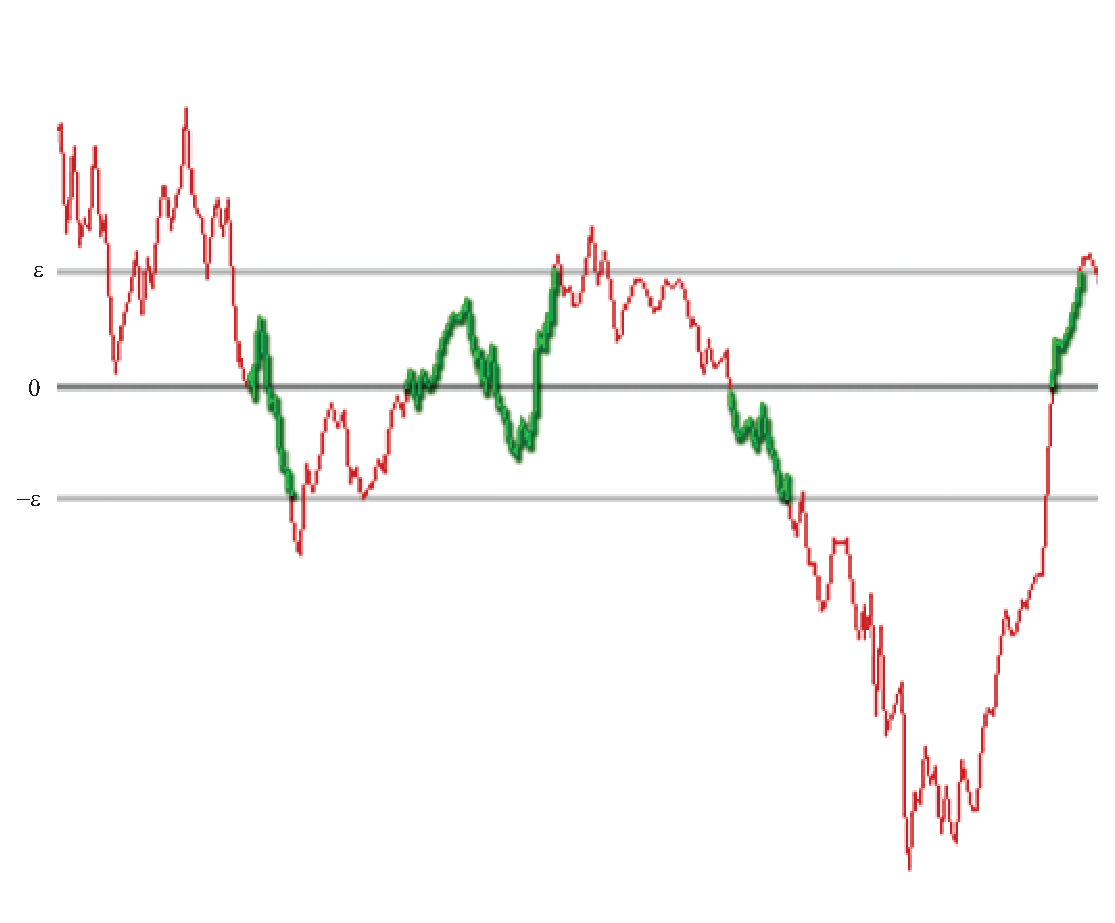
\includegraphics[scale=0.33]{resample1.eps}&
   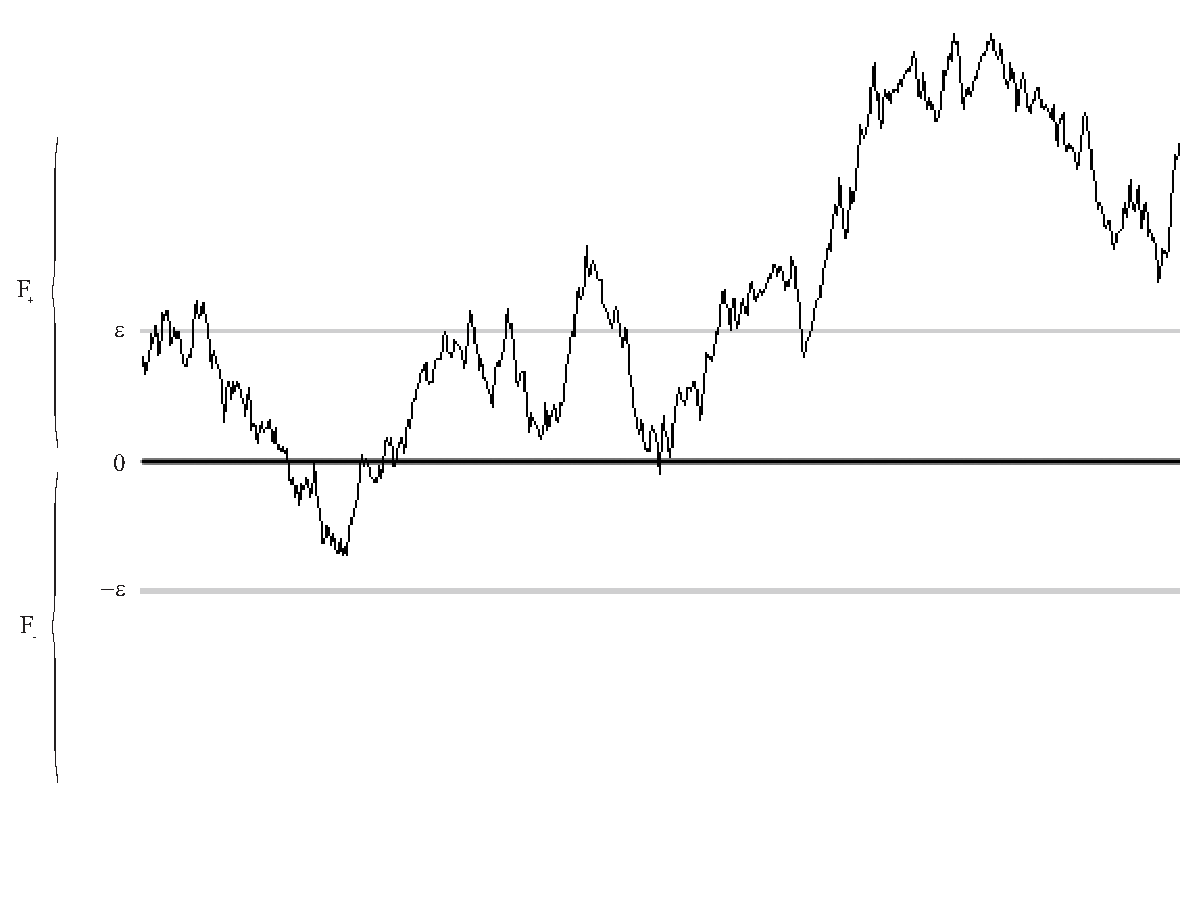
\includegraphics[scale=0.33]{resample2.eps}
   \end{array}$
   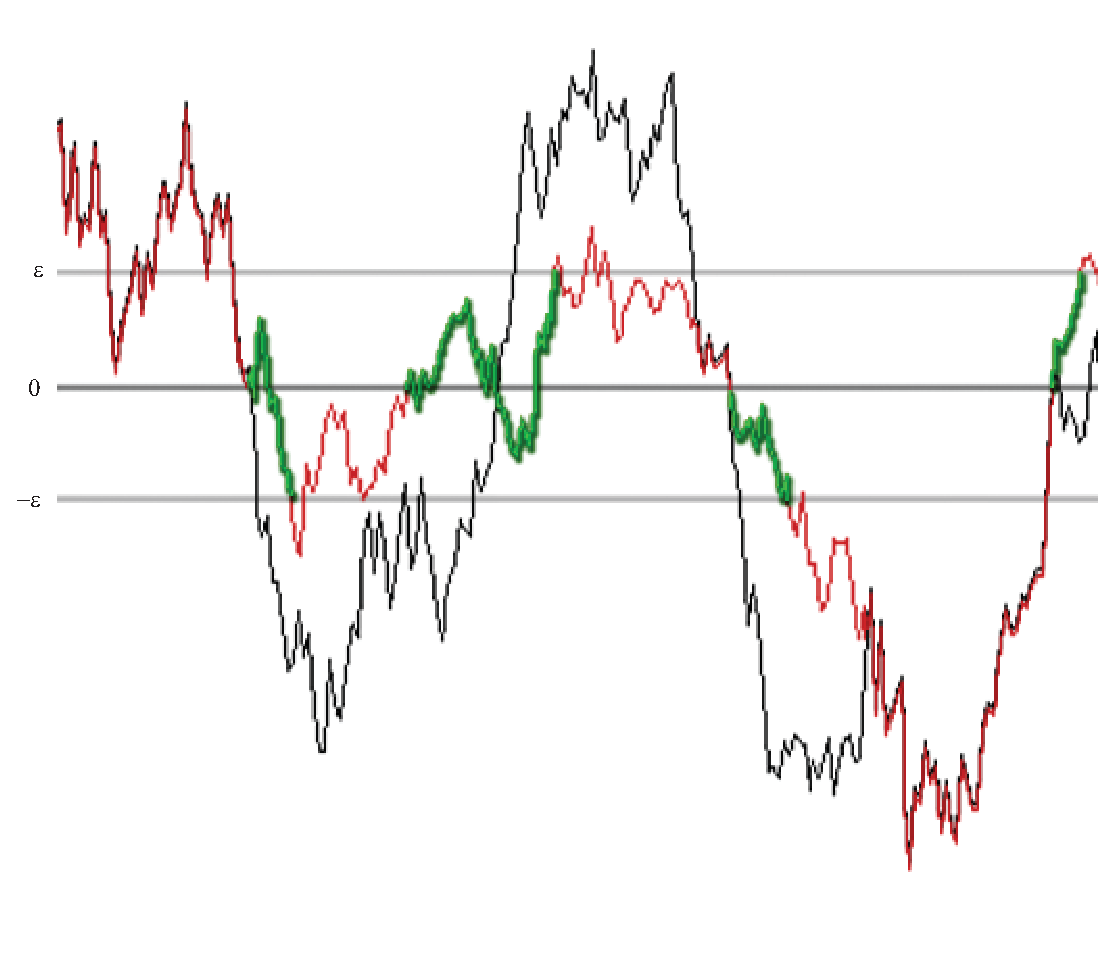
\includegraphics[scale=0.33]{resample.eps}
   \caption{
   A sample of the a web trajectory and the corresponding perturbed processes.
   The top left image depicts the perturbed process, with state B in bold.
   The top right image depicts the original web trajectory. The center image,
   illustrates both processes together, showing the segments where they coalesce.
   }
\end{figure}

The following lemma specifies in what sense the perturbed process is
an approximation of the trajectory of the web.

\begin{lemma}
  \label{lem:resamplede-to-sampled}
  \statementoflemresampledetosampled
\end{lemma}

Lemma \ref{lem:sampled-twostrip-meas} reduces to Lemma
\ref{lem:resamplede-to-sampled}.

\begin{proof}[Proof of reduction]
  $\resamplede$ is $\twostripsreservoir$-measurable, so we use Lemma
  \ref{lem:resamplede-to-sampled} to conclude that $\sampled$ is also
  $\twostripsreservoir$-measurable.  However, since $\sampled$ is
  actually independent of $\reservoir$ we can use a basic result on
  tensor products of Hilbert spaces (for example (1c1), p5 of
  \cite{tsirelson-completion}) to conclude that $\sampled$ is
  in fact $\twostrips$-measurable.
\end{proof}

We devote the following section to the proof of Lemma
\ref{lem:resamplede-to-sampled}.
}
